\documentclass[12pt]{article}  

\usepackage
[colorlinks=true, pdfstartview=FitV, linkcolor=blue, citecolor=blue, urlcolor=blue]
{hyperref}

\usepackage{amssymb}  
\usepackage{amsthm}
\usepackage{amsmath}
\usepackage{graphics} 
\usepackage{graphicx} 
%\usepackage[latin1]{inputenc}
\usepackage{tikz}
\usepackage{pgfplots}
\usepackage{wrapfig}
\usepackage{caption}
\usepgfplotslibrary{polar}
\usepackage{ skull }


% GNUPLOT required
\usepackage{verbatim}

\linespread{1.3}

%\addtolength{\textwidth}{80pt}
\addtolength{\evensidemargin}{20pt}
\addtolength{\oddsidemargin}{20pt}

%%%%%%%%%%%%%%%%%%%%%%%%%%%%%%%%%%%%%%%%%%%%%%
%  Begin user defined commands

\newcommand{\map}[1]{\xrightarrow{#1}}

\newcommand{\N}{\mathbb N}
\newcommand{\Z}{\mathbb Z}
\newcommand{\Primes}{\mathbb P}
\newcommand{\Q}{\mathbb Q}
\newcommand{\R}{\mathbb R}
\newcommand{\C}{\mathbb C}
\newcommand{\bz}{\mathbb Z}
\newcommand{\bq}{\mathbb Q}
\newcommand{\br}{\mathbb R}
\newcommand{\bc}{\mathbb C}
\newcommand{\al}{\alpha}
\newcommand{\be}{\beta}
\newcommand{\ga}{\gamma}
\newcommand{\de}{\delta}
\newcommand{\ep}{\epsilon}
\DeclareMathOperator{\lub}{l.u.b.}
%  End user defined commands
%%%%%%%%%%%%%%%%%%%%%%%%%%%%%%%%%%%%%%%%%%%%%%


%%%%%%%%%%%%%%%%%%%%%%%%%%%%%%%%%%%%%%%%%%%%%%
% These establish different environments for stating Theorems, Lemmas, Remarks, etc.

\newtheorem{Thm}{Theorem}
\newtheorem{Prop}[Thm]{Proposition}
\newtheorem{Lem}[Thm]{Lemma}
\newtheorem{Cor}[Thm]{Corollary}

\theoremstyle{definition}
\newtheorem{Def}[Thm]{Definition}

\theoremstyle{remark}
\newtheorem{Rem}[Thm]{Remark}
\newtheorem{Ex}[Thm]{Example}

\theoremstyle{definition}
\newtheorem{Exercise}{Problem}

\newenvironment{Solution}{\noindent\textbf{Solution.}}{}

%\renewcommand{\labelenumi}{(\alph{enumi})}
\renewcommand\qedsymbol{QED}
% End environments 
%%%%%%%%%%%%%%%%%%%%%%%%%%%%%%%%%%%%%%%%%%%%%%%
%Some commands to save paper


\setlength{\parindent}{0in}
\setlength{\parskip}{8pt}

\DeclareMathOperator{\arcsec}{arcsec}
\DeclareMathOperator{\arccot}{arccot}
\DeclareMathOperator{\arccsc}{arccsc}
\DeclareMathOperator{\LH}{\ \underset{\text{LH}}{=}\ }
\newcommand{\Dep}{\Delta_+}
\newcommand{\Dem}{\Delta_-}
\newcommand{\bu}{\mathbf u}
\newcommand{\bv}{\mathbf v}
\newcommand{\bw}{\mathbf w}

\newcommand{\ora}{\overrightarrow}



\addtolength{\textwidth}{80pt}
\addtolength{\evensidemargin}{-40pt}
\addtolength{\oddsidemargin}{-40pt}
\addtolength{\topmargin}{-80pt}
\addtolength{\textheight}{1.8in}

\setlength{\parindent}{0in}
\setlength{\parskip}{8pt}

\DeclareMathOperator{\arcsinh}{arcsinh}

%%%%%%%%%%%%%%%%%%%%%%%%%%%%%%%%%%%%%%%%%%%%%%
% Now we're ready to start
%%%%%%%%%%%%%%%%%%%%%%%%%%%%%%%%%%%%%%%%%%%%%%

\begin{document}  

%\author{Your Name}
{\bf MATH 1103 Homework 2}\\
{\bf Due Friday February 2, 2018}


Practice Problems (not to be turned in)

\vskip5pt
{\bf Practice 1.\ } Use the Geometric Expansion to prove the equality of decimals
\[.99999\dots=1.\]
[Recall that 
$.99999\dots=\lim\limits_{n\to\infty}\left(\dfrac{9}{10}+\dfrac{9}{10^2}+\cdots+\dfrac{9}{10^n}\right).$
]
%\begin{Solution}
%Set $x=.99999\dots$.  We know that $x\leq 1$. Suppose $x<1$. 
%Let $\ep$ be an arbitrary positive number. Adding $\ep$ to $x$ will cause a $1$ to carry over to the left of the decimal point, so $1\leq x+\ep$. 
%Therefore $ x< 1\leq x+\ep$, so $1-x<\ep$. By the $\ep$ theorem, we have $x=1$. 
%\end{Solution}

{\bf Practice 2.\ }   If humans  had just two fingers, they would express all numbers in binary expansions instead of decimals. Even though they usually have ten fingers,  humans designed computers to express numbers in binary expansions. 

For simplicity, suppose $r$ is a number such that $0<r<1$.
The {\bf binary expansion} of $r$ is 
\[r=.a_1a_2a_3\dots, \]
where each $a_k$ is either $0$ or $1$ and the precise meaning of the expression with $\dots$ is 
\[.a_1a_2a_3\cdots
=\lim_{n\to\infty} \left(\frac{a_1}{2}+\frac{a_2}{2^2}+\cdots+\frac{a_n}{2^n}\right).
\]
For example, the binary expansion of $1/2=.1000\cdots$. 
Just as with decimals, the binary expansion is based on the Geometric Expansion. 

a) Verify the binary expansion
\[\frac{1}{3}= .0101010101\dots
\]

b) Find the binary expansion of $1/13$.


{\bf Practice 3.\ } (Challenging) Prove that a convergent sequence is bounded. 
[Hint: take $\ep=1$ in the definition of convergence, and consider $x_n$ for $n< N$ and $n\geq N$, where $|x-x_n |<1$ for $n\geq N$. ]

 \rule{\textwidth}{1pt}
The homework to be turned in may be found on the next page.
\newpage

{\bf Homework to be turned in.}

{\bf 1.\ } A chessboard has 64 squares. Put one grain of rice on the first square, half-a grain of rice on the second square, a fourth of a grain on the third square, an eighth of a grain on the fourth square, and so on for all 64 squares. 
Find the fraction, in lowest terms, of grains of rice on the entire square.  Is this fraction more or less than two grains of rice?
%\begin{Solution} 
%\end{Solution}

\vskip10pt

{\bf 2.\ } Prove that the sequence $(x_n)$ given by
\[x_n=\frac{1\cdot 3\cdot 5\cdots (2n-1)}{2\cdot 4\cdot 6\cdots (2n)}\]
converges. (You don't have to find the limit.) 

%\begin{Solution} Squeeze-Law, or Bounded-Times Zero.
%\end{Solution} 

{\bf 3.\ } Prove that the sequence $(x_n)$ given by
\[x_n=\frac{1}{n+1}+\frac{1}{n+2}+\frac{1}{n+3}+\cdots+\frac{1}{n+n}\]
converges and the limit is somewhere between $0$ and $1$. 
%\begin{Solution} Squeeze-Law, or Bounded-Times Zero.
%\end{Solution} 

More problems on the next page. 
\newpage
\rule{\textwidth}{1pt}
Around the time Isaac Newton was born (1642), Pierre de Fermat (a French judge) determined the area $A$ under the graph of $y=x^p$ above an interval of the form $0\leq x\leq a$, where $p$ is any positive integer (thus improving on Archimedes, who did the case $p=2$, as we saw on the last hw).  Fermat used only the Geometric Series. You will follow Fermat's footsteps in the next few problems. 

Let $r$ be any number such that $0<r<1$, and let $n$ be a positive integer.   
Divide the interval $[0,a]$ into $n+1$ sub-intervals 
\[I_n=[0,ar^n],\quad I_{n-1}=[ar^n,ar^{n-1}],\quad I_{n-2}=[ar^{n-1}, ar^{n-2}],\quad \dots,\quad  I_1=[ar^2,ar],\quad I_0=[ar,a].\]
(See pictures below.)

\rule{\textwidth}{1pt}

{\bf 4.\ } Find the total area of these rectangles below the graph (there is no rectangle above $I_n$) and compute the limit of this area as $n\to\infty$.  Call this limit $L(r)$ ($L$ for ``Lower"). 

\begin{center}
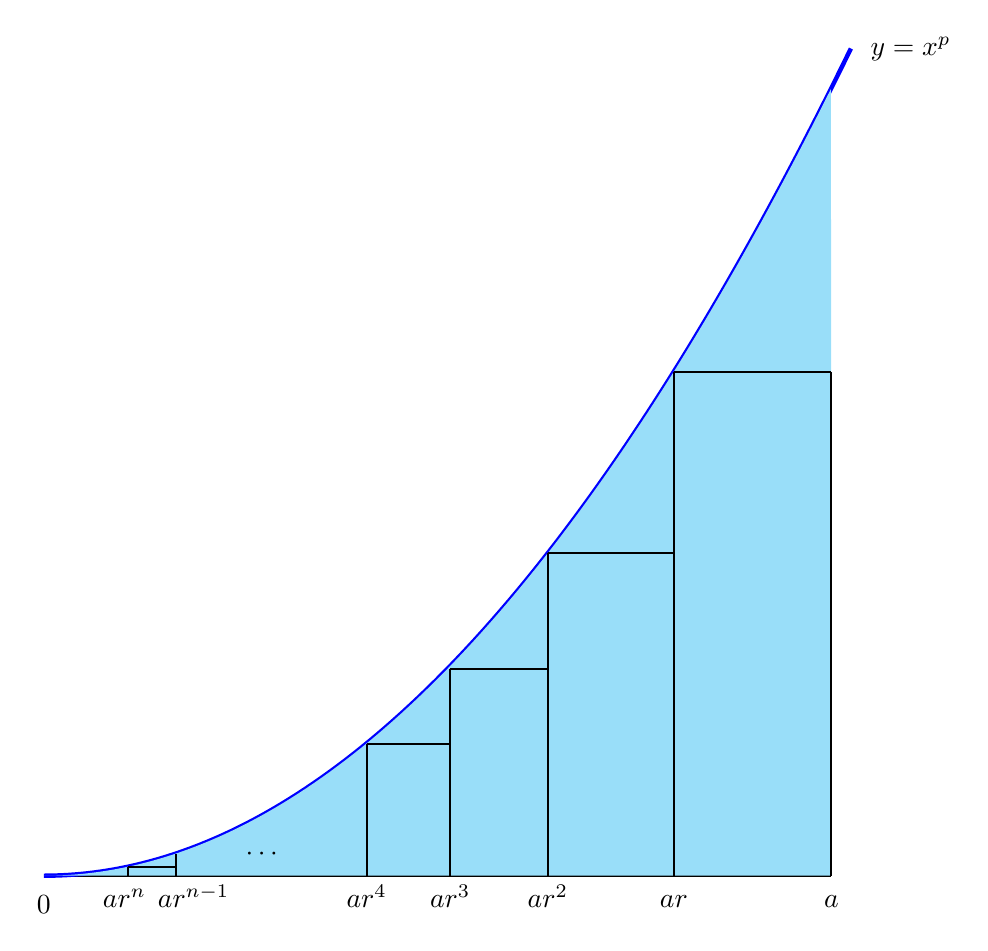
\begin{tikzpicture}[samples=100, domain=0:4, scale=2.5]
\draw[black,   thick] (0,0) -- (4,0 );%a=4
\draw[blue, ultra thick] plot [domain=0: 4.1 ] (\x,{(1/4)*\x*\x)}) ;
\fill[fill=cyan!40!](0,0) -- plot [domain=0:4, ] (\x,{(1/4)*\x*\x)}) -- (4,0) -- cycle;
\draw [black,  thick] (4,0) -- (4,.64*4);

\node[label=right: {$y=x^p$}] at (4.1,4.2) {};
%\node[label=right:
%{$a^{p+1}\cdot \dfrac{r^p}{1+r+\cdots+r^p}\ \leq\ \text{Area}\ \leq \ 
%\dfrac{a^{p+1}}{1+r+\cdots+r^p}$}
%] at (0,3.5) {};

\node[label=below: $0$] at (0,0) {};
\node[label=below: $a$] at (4,0) {};

\node[label=below: $ar$] at (.8*4,0) {}; %r=.8
\draw [black,  thick] (.8*4,0) -- (.8*4,.64*4);
\draw [black,  thick] (.8*4,.64*4) -- (4,.64*4);

\node[label=below: $ar^2$] at (.64*4,0.05) {};
\draw [black,   thick] (.64*4,0) -- (.64*4,.41*4);
\draw [black,  thick] (.64*4,.41*4) -- (.8*4,.41*4);

\node[label=below: $ar^3$] at (.516*4,0.05) {};
\draw [black,  thick] (.516*4,0) -- (.516*4,.2621*4);
\draw [black,  thick] (.516*4,.2621*4) -- (.64*4,.2621*4);

\node[label=below: $ar^4$] at (.41*4,0.05) {};
\draw [black,  thick] (.41*4,0) -- (.41*4,.1677*4);
\draw [black,  thick] (.41*4,.1677*4) -- (.516*4,.1677*4);

\node[label=below: $\cdots$] at (.2621*4+.07,.06*4) {};

\node[label=below: $ar^{n-1}$] at (.1677*4+.09,0.05) {};
\draw [black,  thick] (.1677*4,0) -- (.1677*4,.028*4);
%\draw [black,  thick] (.1073*4,.028*4)-- (.1677*4,.028*4);

\node[label=below: $ar^n$] at (.1073*4-.02,0.03) {};
\draw [black,  thick] (.1073*4,0) -- (.1073*4,.011*4);
\draw [black,  thick] (.1073*4,.011*4) -- (.167*4,.011*4);
%\draw [red,  thick] (.1073*4,.011*4) -- (0,.011*4);
%\draw [red,  thick] (0,0) -- (0,.011*4);
%\draw [red,  thick] (0,0) -- (.1073*4,0);
% 8^3=.512, .8^4=.4096, .8^5=.3277, .8^6=.2621, 
% .8^6=.1677,  .8^10=.1073, .8^12=.0687, .8^14=.044, 
%.8^16=.028, .8^18=.018, .8^20=.011
%
% y=x^2/4
\end{tikzpicture}
\end{center}


\newpage
{\bf 5.\ } Find the total area of these rectangles above the graph (including the little red rectangle above $I_n$) and take the limit of this area as $n\to\infty$. Call this limit $U(r)$ ($U$ for ``Upper").

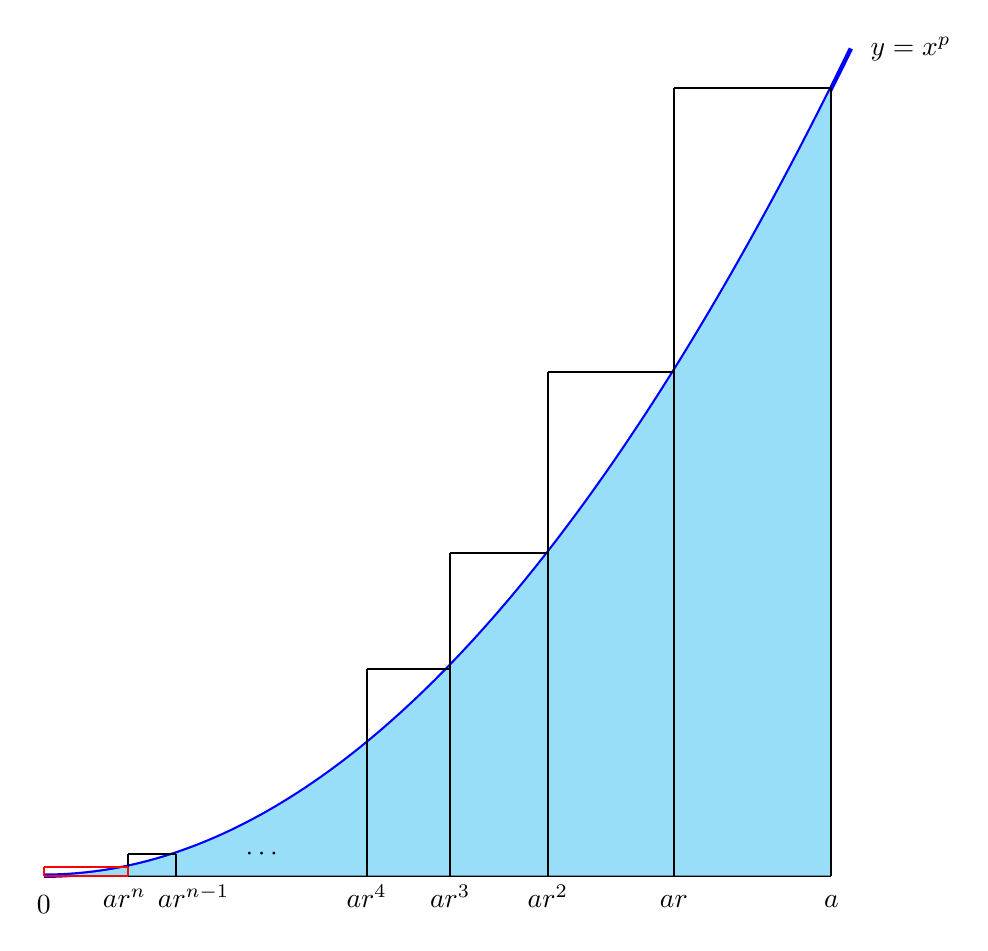
\begin{tikzpicture}[samples=100, domain=0:4, scale=2.5]
\draw[black,   thick] (0.073*4,0) -- (4,0 );%a=4
\draw[blue, ultra thick] plot [domain=0: 4.1 ] (\x,{(1/4)*\x*\x)}) ;
\fill[fill=cyan!40!](0,0) -- plot [domain=0:4, ] (\x,{(1/4)*\x*\x)}) -- (4,0) -- cycle;
\draw [black,  thick] (4,0) -- (4,4);

\node[label=right: {$y=x^p$}] at (4.1,4.2) {};

\node[label=below: $0$] at (0,0) {};
\node[label=below: $a$] at (4,0) {};

\node[label=below: $ar$] at (.8*4,0) {}; %r=.8
\draw [black,  thick] (.8*4,0) -- (.8*4,4);
\draw [black,  thick] (.8*4,4) -- (4,4);

\node[label=below: $ar^2$] at (.64*4,0.05) {};
\draw [black,   thick] (.64*4,0) -- (.64*4,.64*4);
\draw [black,  thick] (.64*4,.64*4) -- (.8*4,.64*4);

\node[label=below: $ar^3$] at (.516*4,0.05) {};
\draw [black,  thick] (.516*4,0) -- (.516*4,.4096*4);
\draw [black,  thick] (.516*4,.4096*4) -- (.64*4,.4096*4);

\node[label=below: $ar^4$] at (.41*4,0.05) {};
\draw [black,  thick] (.41*4,0) -- (.41*4,.2621*4);
\draw [black,  thick] (.41*4,.2621*4) -- (.516*4,.2621*4);

\node[label=below: $\cdots$] at (.2621*4+.07,.06*4) {};

\node[label=below: $ar^{n-1}$] at (.1677*4+.09,0.05) {};
\draw [black,  thick] (.1677*4,0) -- (.1677*4,.028*4);
\draw [black,  thick] (.1073*4,.028*4)-- (.1677*4,.028*4);

\node[label=below: $ar^n$] at (.1073*4-.02,0.03) {};
\draw [black,  thick] (.1073*4,0) -- (.1073*4,.028*4);
\draw [red,  thick] (.1073*4,0) -- (.1073*4,.011*4);
\draw [red,  thick] (.1073*4,.011*4) -- (0,.011*4);
\draw [red,  thick] (0,0) -- (0,.011*4);
\draw [red,  thick] (0,0) -- (.1073*4,0);
% 8^3=.512, .8^4=.4096, .8^5=.3277, .8^6=.2621, 
% .8^6=.1677,  .8^10=.1073, .8^12=.0687, .8^14=.044, 
%.8^16=.028, .8^18=.018, .8^20=.011
%
% y=x^2/4
\end{tikzpicture}



{\bf 6.\ } From the pictures, we have $L(r)<A<U(r)$.  Compute the limits of $L(r)$ and $U(r)$ as $r\to 1$ and 
thereby compute $A$ as Fermat did. 
\vskip5pt
%\begin{Solution} 
%\end{Solution}

\end{document}

 
 
